%% -*- coding: utf-8 -*-
\documentclass[12pt,a4paper]{scrartcl} 
\usepackage[utf8]{inputenc}
\usepackage[english,russian]{babel}
\usepackage{indentfirst}
\usepackage{misccorr}
\usepackage{graphicx}
\usepackage{amsmath}
\usepackage{float}
\usepackage{ dsfont }

\usepackage{xcolor}
\usepackage{hyperref}
\hypersetup{colorlinks,
  pdftitle={The title of your document},
  pdfauthor={Your name},
  allcolors=[RGB]{000 000 000}}

\begin{document}
\begin{titlepage}
  \begin{center}

    Санкт-Петербургский политехнический университет Петра Великого

    \vspace{0.25cm}
    
    Институт прикладной математики и механики
    
    Кафедра «Прикладная математика»
    \vfill

	\vspace{0.25cm}
	    Отчёт\\
	по лабораторной работе №3\\
	по дисциплине\\
	«Вычислительные комплексы»

  \bigskip

\end{center}
\vfill

\newlength{\ML}
\settowidth{\ML}{«\underline{\hspace{0.7cm}}» \underline{\hspace{2cm}}}
\hfill\begin{minipage}{0.4\textwidth}
  Выполнил студент\\ В.\,А.~Рыженко\\
\end{minipage}%
\bigskip

\hfill\begin{minipage}{0.4\textwidth}
  Проверил:\\
к.ф.-м.н., доцент\\
Баженов Александр Николаевич\\
\end{minipage}%
\vfill

\begin{center}
  Санкт-Петербург, 2020 г.
\end{center}
\end{titlepage}

\tableofcontents
%\listoffigures
\newpage


\section{Постановка задачи}

Требуется решить недоопределённую интервальную систему линейных алгебраических уравнений (ИСЛАУ) с матрицей 3×2 и переопределённую ИСЛАУ с матрицей 2×3. Используемые матрицы должны совпадать с точностью до транспонирования. Для случая 3х2 построить график $Tol(x_1, x_2)$. Для случая 2x3 проанализировать решение. Построить 3-мерный образ допускового множества или его проекции на плоскости $(x_i O x_j)$. Найти допусковое множество решений, оценку вариабельности решения ive для обоих случаев.


\subsection{Конкретизация задачи и метод решения}
\subsubsection{Переопределенная ИСЛАУ}
	В качестве исходной матрицы СЛАУ была выбрана точечная матрица $A$ и вектор $x$:
	
	\begin{equation}
		A = \left(
		\begin{array}{cc}
		14 & 13 \\
		18 & 21\\
		16 & 7
		\end{array}
		\right),
		x = \left(
		\begin{array}{c}
		0.3 \\
		0.1
		\end{array}
		\right)
		\label{eq:A_x_1}
	\end{equation}

	Таким образом, правая часть СЛАУ была определена значениями $A$ и $x$ (\ref{eq:A_x_1})

	\begin{equation}
		b = A \cdot x = \left(
		\begin{array}{c}
		5.5 \\
		7.5 \\
		5.5
		\end{array}
		\right)
		\label{eq:b_1}
	\end{equation}

	Далее, положим величины радиусов элементов $rad A$ и $rad b$ равными

	\begin{equation}
		rad A = \left(
		\begin{array}{cc}
		2 & 2 \\
		2 & 3\\
		1 & 1
		\end{array}
		\right),
		rad b = \left(
		\begin{array}{c}
		1.5 \\
		2 \\
		2
		\end{array}
		\right)
		\label{eq:rad_A_b_1}
	\end{equation}

	Из (\ref{eq:A_x_1}), (\ref{eq:b_1}), (\ref{eq:rad_A_b_1}) имеем переопределенную ИСЛАУ 3 × 2

	\begin{equation}
		rad A = \left(
		\begin{array}{cc}
		(12, 16) & (11, 15) \\
		(16, 20) & (18, 24) \\
		(15, 17) & (6, 8)
		\end{array}
		\right) \cdot 
		x = \left(
		\begin{array}{c}
		(3, 6) \\
		(4, 8) \\
		(2, 6)
		\end{array}
		\right).
		\label{eq:islau_1}
	\end{equation}

\subsubsection{Недоопределенная ИСЛАУ}

Для задания ИСЛАУ матрица $A$ (\ref{eq:A_x_1}) из предыдущего раздела была транспонирована, а
вектор $x$ дополнен ещё одним членом:

\begin{equation}
		A = \left(
		\begin{array}{ccc}
		14 & 18 & 16\\
		13 & 21 & 7
		\end{array}
		\right),
		x = \left(
		\begin{array}{c}
		0.3 \\
		0.1 \\
		0.2
		\end{array}
		\right)
		\label{eq:A_x_2}
	\end{equation}

	Для них была определена правая часть:

	\begin{equation}
		b = A \cdot x = \left(
		\begin{array}{c}
		9.2 \\
		7.4
		\end{array}
		\right)
		\label{eq:b_2}
	\end{equation}

	Далее, аналогично (\ref{eq:islau_1}), была получена ИСЛАУ:

	\begin{equation}
		rad A = \left(
		\begin{array}{ccc}
		(12, 16) & (16, 20) & (15, 17) \\
		(11, 15) & (18, 24) & (6, 8)
		\end{array}
		\right) \cdot 
		x = \left(
		\begin{array}{c}
		(7, 12) \\
		(5, 8)
		\end{array}
		\right).
		\label{eq:islau_2}
	\end{equation}

\subsubsection{Исследование разрешимости}

	Для исследования разрешимости этих интервальной ИСЛАУ использовался распознающий функционал $Tol (x)$:

	\begin{equation}
		Tol(x) = \min_{1 \leq i \leq n}{(radb_i - |midb_i - \sum_{j=1}^m{a_{ij}x_j}|)}
	\end{equation}

	Допусковое множество решений ИСЛАУ при этом задаётся условием $Tol(x) \geq 0$. Таким образом для нахождения 	допускового множества и проверки разрешимости системы удобно найти точку $x$, максимизирующую распознающий функционал, и рассмотреть её окрестность.

\subsubsection{Оценка меры вариабельности}

	Оценка меры вариабельности ive была найдена по формуле:
	
	\begin{equation}
		ive(\bold{A}; \bold{b}) = \sqrt{n}(\min_{A \in \bold{A}}{A}*||argmax{Tol})|| \cdot \frac{max Tol}{||b||}
		\label{eq:ive}
	\end{equation}

	Брус оценки 	$\tilde x$ :
	
	\begin{equation}
		\tilde x = [argmax Tol - ive, argmax Tol + ive]
		\label{eq:brus}
	\end{equation}


\section {Реализация}
Лабораторная работа выполнена с помощью встроенных средств языка программирования Matlab и Python. Так как используемые методы оценок — интервальные, необходимым оказалось также привлечение библиотеки INTLAB для поддрежки арифметических операций в интревальной арифметике. Программы И.А. Шарой IntLinInc2D и IntLinInc3D использовались для визуализации множества интервальных и точечных систем линейных отношений.
Для нахождения экстремума распознающего функционала использована программа tolsolvty для Python.

\section {Результаты}

\subsection{Переопределенная ИСЛАУ}

Минимальное число обусловленности матрицы ИСЛАУ (\ref{eq:islau_1}):

\begin{equation}
	C_{min} = \min{condA} = 5.0504
\end{equation}

Минимум достигался на матрице:
\begin{equation}
	\left(
	\begin{array}{cc}
	16 & 15 \\
    	20 & 24 \\
    	17 & 6
	\end{array}
	\right)
\end{equation}

С помощью программы $tolsolvty$ были найдены максимум функционала распознающего функционала $max Tol$ и значение аргумента, в которой он достигался $arg max Tol$.

\begin{equation}
	\begin{array}{c}
	maxTol = 0.85135 \\
	argmaxTol = (0.28378, 0.04054)^T
	\end{array}
\end{equation}

В случае переопределённой ИСЛАУ с не слишком широкими интервалами максимум распознающего функционала обычно будет отрицательным, а допусковое множество, соответственно, пустым, что означает несовместность системы. В рассматриваемом случае, однако, матрица и вектор правой части были подобраны так, чтобы решение существовало. Так как искомы вектор $x$ в этом случае содержит всего две компоненты, допусковое множество можно изобразить, как область на плоскости $x_1$ x $x_2$.

Оценка меры вариабельности ive (\ref{eq:ive})

\begin{equation}
	ive(\bold{A}; \bold{b}) = 0.41014
\end{equation}

Брус оценки $\tilde x$ (\ref{eq:brus}):

\begin{equation}
	\tilde x = ([0.07871, 0.48885], [-0.16452, 0.24561])^T
\end{equation}

Результат графического представления полученного бруса, множества решений и их совмещения.

\begin{figure}[H]
    \centering
    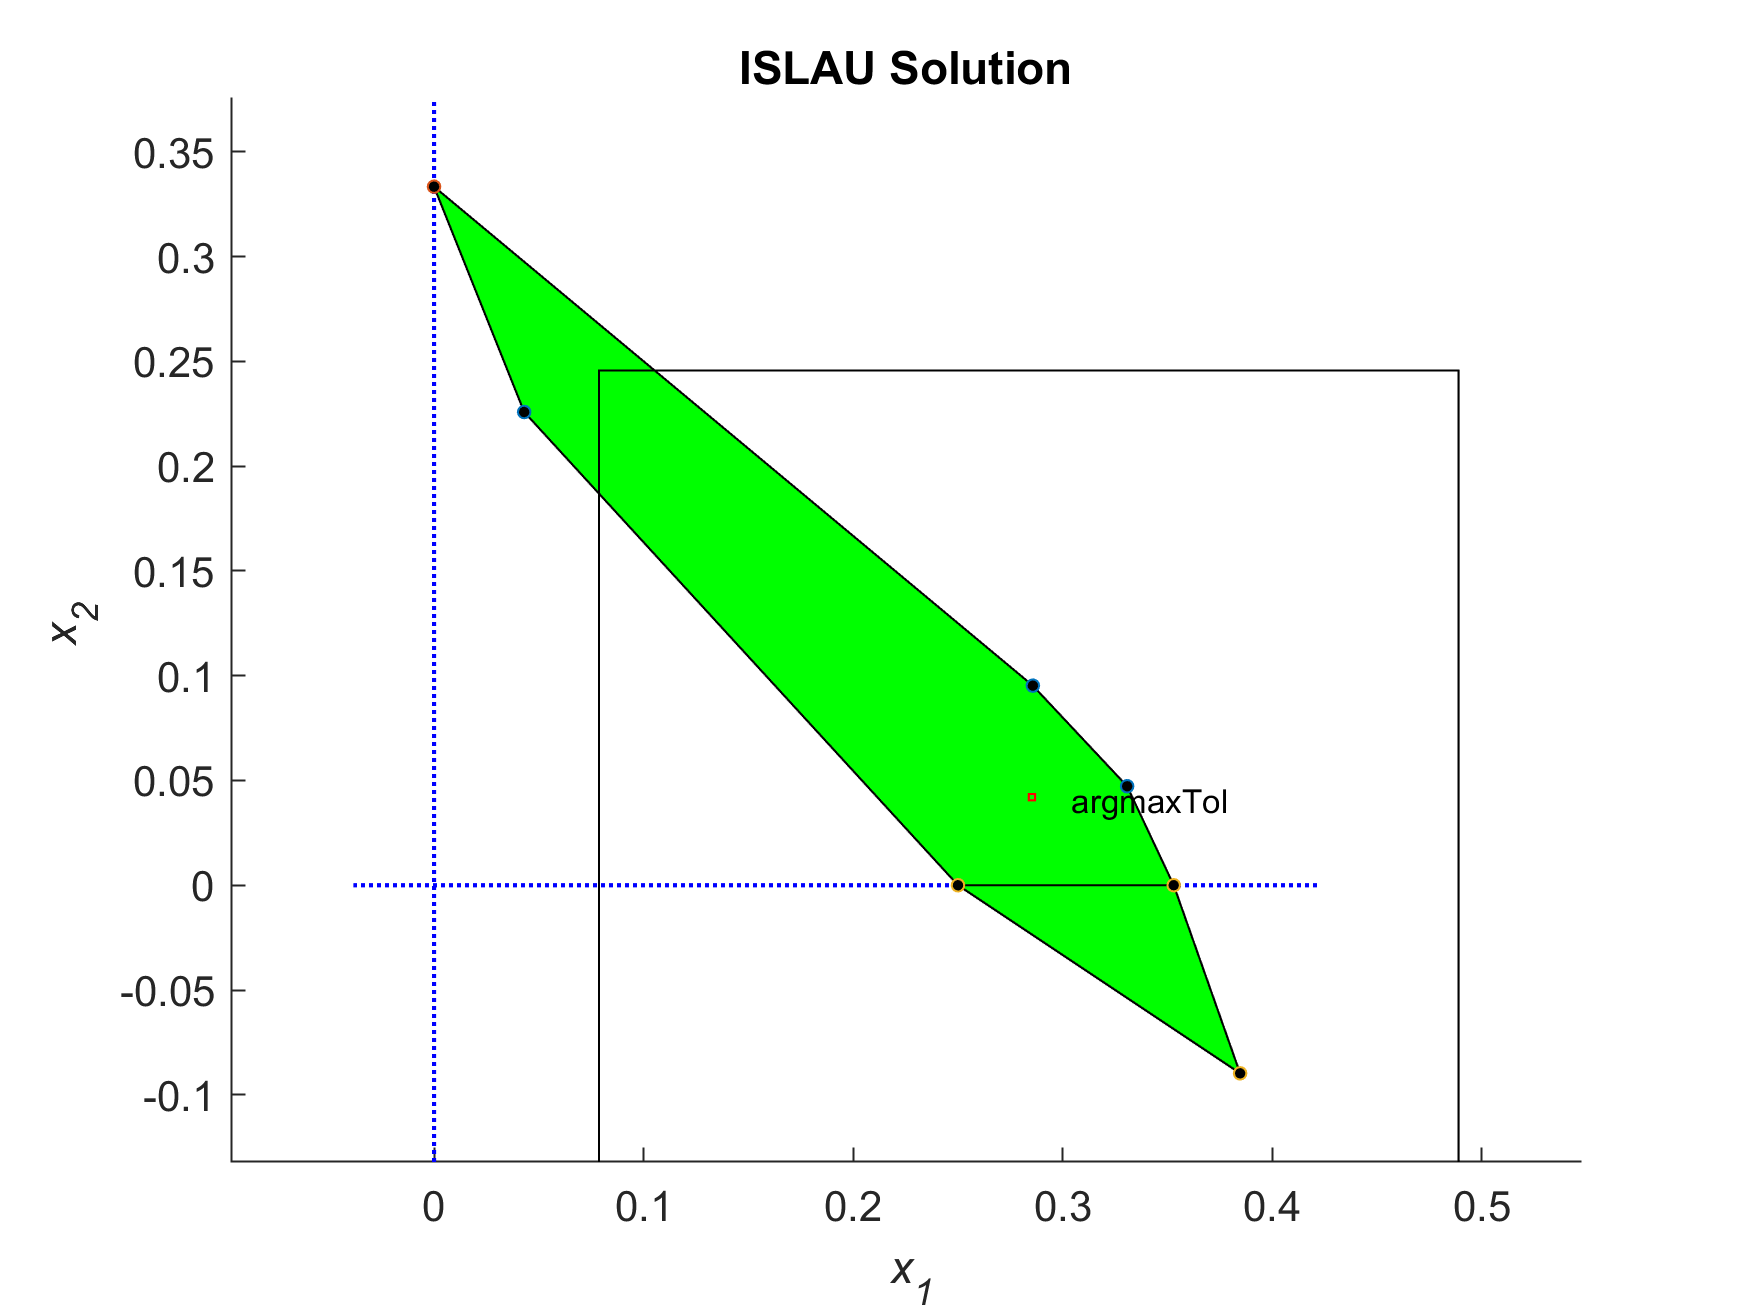
\includegraphics[width=10cm, height=8cm]{fig/ISLAU_1.png}
    \caption{Зелёным цветом изображено допусковое множество решений, чёрный квадрат - брус $ive$, красная точка - достигался максимум функционала.}
\end{figure}

Далее представлен график распознающего функционала.

\begin{figure}[H]
    \centering
    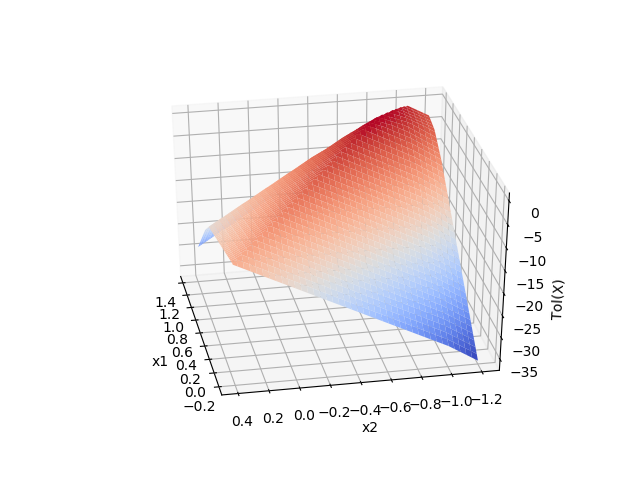
\includegraphics[width=10cm, height=8cm]{fig/Tol.png}
    \caption{Расознающий функционал}
\end{figure}

\subsection{Недоопределенная ИСЛАУ}

При транспонировании матрицы число обусловленности не меняется

\begin{equation}
	C_{min} = \min{condA} = 5.0504
\end{equation}

С помощью программы $tolsolvty$ были найдены максимум функционала распознающего функционала $max Tol$ и значение аргумента, в которой он достигался $arg max Tol$.

\begin{equation}
	\begin{array}{c}
	maxTol = 1 \\
	argmaxTol = (1.394 \cdot 10^{-6}, 0.231, 0.306)^T
	\end{array}
\end{equation}

Оценка меры вариабельности ive (\ref{eq:ive})

\begin{equation}
	ive(\bold{A}; \bold{b}) = 0.47586
\end{equation}

Брус оценки $\tilde x$ (\ref{eq:brus}):

\begin{equation}
	\tilde x = ([-0.23793	0.23793], [-0.00651,	0.46934], [0.06782, 0.54369])^T
\end{equation}

Результат графического представления полученного бруса, множества решений и их совмещения.

\begin{figure}[H]
    \centering
    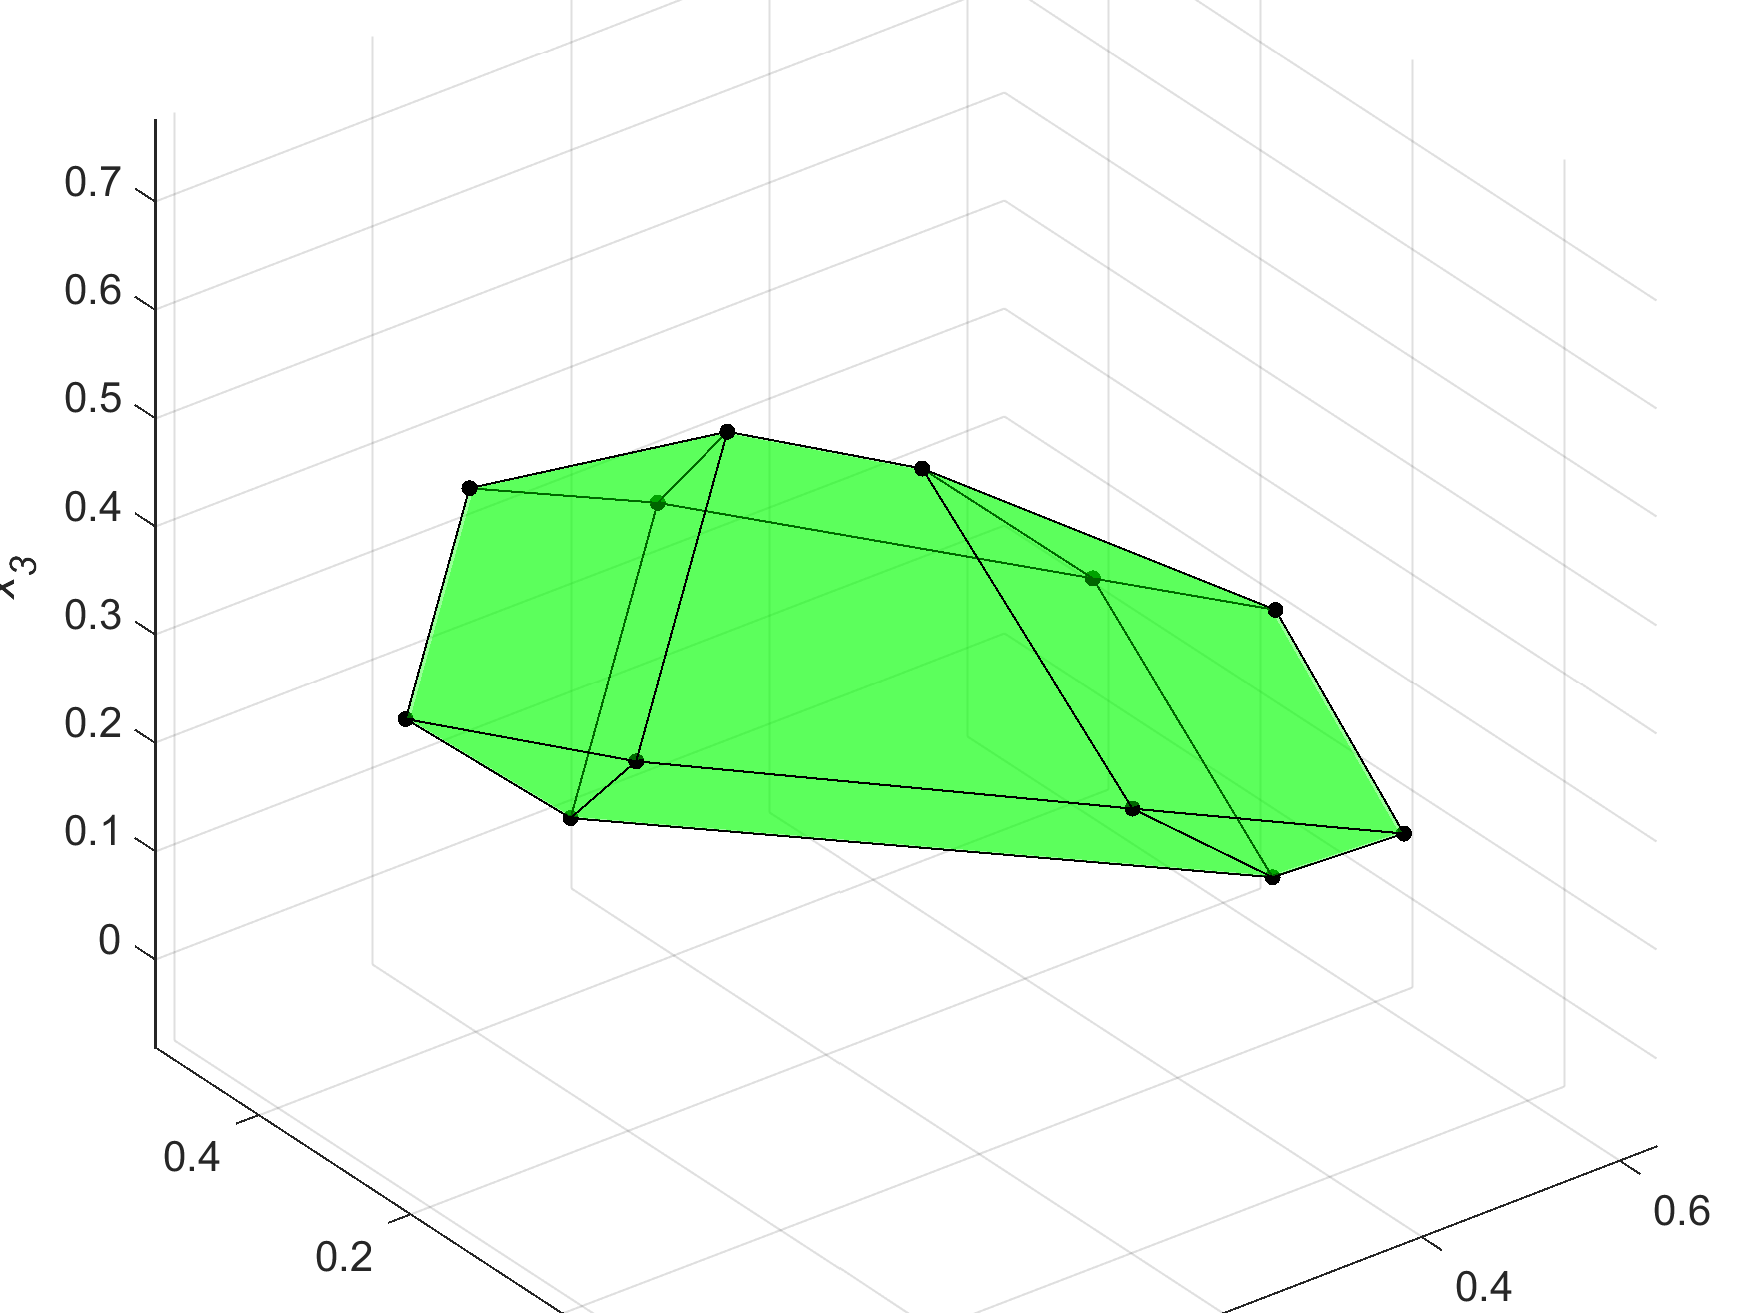
\includegraphics[width=10cm, height=8cm]{fig/ISLAU_2_3D.png}
    \caption{Зелёным цветом изображено допусковое множество решений}
\end{figure}

Заметим, что $argmaxTol$ заметно отличается от $x_0$. При этом $argmaxTol$ всё же удовлетворяет границам правой части (\ref{eq:islau_2}), $A\cdot argmaxTol \subseteq b$. Такой результат - проявление неоднозначности решения обратной задачи. При этом для СЛАУ, которая в неинтервальной постановке имела бы бесконечное множество решений, методами интервального анализа получено конечное множество решений.

\section{Приложения}
Репозиторий на GitHub с релизацией: \href{https://github.com/WiillyWonka/Intervals}{github.com}.
\end{document}
